\documentclass[11pt,letterpaper]{article} %Formato general del document
\usepackage[spanish]{babel} % Idioma
\usepackage[utf8]{inputenc} % Codificacion
\usepackage{graphicx} % Agregar figuras(imagenes)
\usepackage{float} % Solucion para imagenes flotantes
\usepackage{listings} % Importar codigos fuente

\title
{
  \textbf{Universidad de Guadalajara}\\
  Departamento de Electrónica\\
  \begin{figure}[H]
    \centering
    
\includegraphics[width=7cm]{figures/UDG_byn.png}
  \end{figure}
  \textbf{Proyecto final}\\
  Procesador de 8 bits\\
  \textit{Sistemas reconfigurables}\\
}
\author{Eduardo Vázquez Díaz\\lalohao@gmail.com}

\begin{document}

\maketitle
\newpage

\tableofcontents
\newpage

\begin{abstract}
  Se construyó un procesador de 8 bits con funcionalidades basicas, utilizando
  verilog y software libre para diseñar y simularlo. Posteriormente se
  implementó en una tarjeta fpga spartan 3.
\end{abstract}

\section{Introducción}
El lenguaje de descripcion de hardware es una potente herramienta que facilita
la creacion de prototipos electronicos. Permite expresar en un lenguaje
sintactico, entendible para los humanos funciones especificas que pueden ser
asignadas a un \emph{FPGA} y cambiarlas las veces que se desee. Un ejemplo de
estos lenguajes es \emph{Verilog}, que es ademas el elegido para llevar a cabo
el diseño que se mostrará mas adelante.
\\ \\
Del software libre (SL) se obtiene otra gran ventaja. La mayoria del software es
documentado y respaldado por una comunidad. GNU/Linux es el mejor ejemplo donde
grandes comunidades se desenvuelven entorno al desarrollo y uso de SL y a la
filosofia que estas transmiten.
\\ \\
Siendo los procesadores la unidad central de practicamente cualquier dispositivo
inteligente, es imprescindible conocer su arquitectura interna y ser capaz de
construir modelos de ellos.


\section{Desarrollo}
El procesador se puede descomponer en unidades mas pequeñas que realizan
especificas tareas.
\begin{figure}[H]
  \centering
  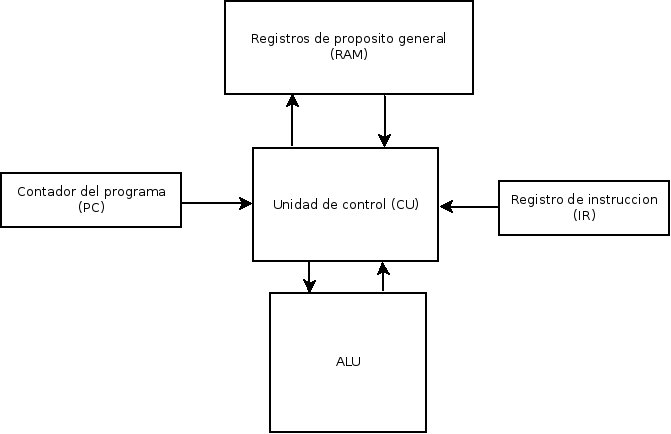
\includegraphics[width=14cm]{figures/bloques.png}
  \caption{Diagrama de bloques del procesador}
\end{figure}

\subsection{Unidad de Control}
El corazon del CPU, la \textbf{unidad de control} se diseño como una maquina de
estados para facilitar su implementacion en el FPGA.
\begin{figure}[H]
  \centering
  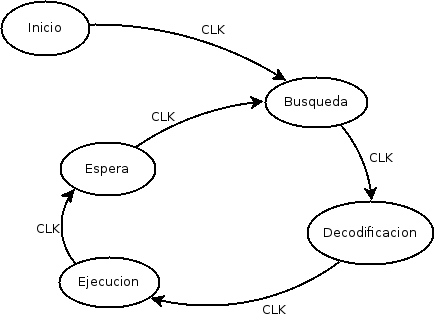
\includegraphics[width=10cm]{figures/cpu_estados.png}
  \caption{Diagrama de estados de la unidad de control (CU)}
\end{figure}
\textbf{Estados}\\
\textbf{Inicio}: Las variables y conexiones internas se (re)inicializan a 0. \\
\textbf{Busqueda}: Se pasa la instruccion completa al IR.\\
\textbf{Decodificacion}: Se prepará para la ejecucion de la instruccion. \\
\textbf{Ejecucion}: Se ejecuta la instruccion. \\
\textbf{Espera}: Se espera a que se termine de ejecutar la instruccion. \\
\begin{figure}[H]
  \centering
  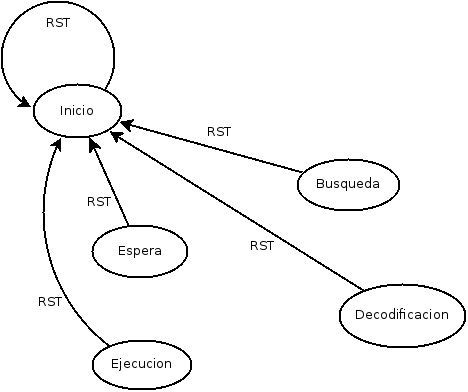
\includegraphics[width=10cm]{figures/cpu_rst.png}
  \caption{Al activar RST todos los estados llevan al inicial.}
\end{figure}

\subsection{Registro de instruccion (IR)}
La idea de enviarle instrucciones a la tarjeta spartan \textbf{xc3s200}
utilizando sus DIP SWITCH conllevo al diseñó de un IR de 8bits.
\begin{figure}[H]
  \centering
  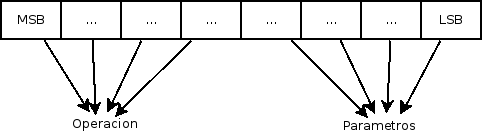
\includegraphics[width=12cm]{figures/instruccion.png}
  \caption{Los 4 bits mas significativos representan la operacion a realizar, con un total de 16 operaciones posibles. Los 4 bits menos significativos son el parametro de la operacion.}
\end{figure}
\begin{figure}[H]
  \centering
  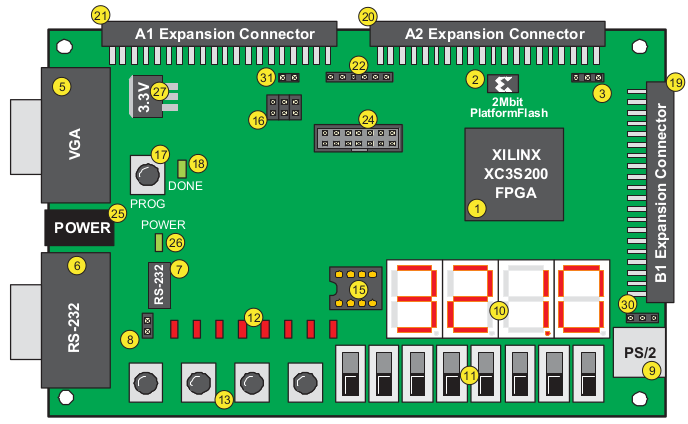
\includegraphics[width=14cm]{figures/s3.png}
  \caption{(11) Cada DIP-Switch representa un bit del IR. (13) CLK manual y reset.}
\end{figure}

\subsection{Registros (Memoria RAM)}
\label{subsec:label}
La memoria RAM cuenta con 16 registros de proposito general de 4 bits cada uno,
lo que permite utilizar la misma longitud para el bus de datos y el bus de
direccion.\\
\begin{figure}[H]
  \centering
  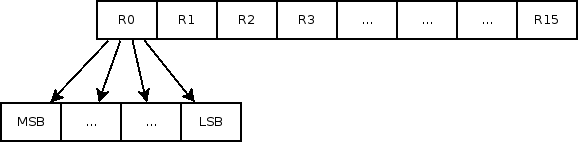
\includegraphics[width=12cm]{figures/ram.png}
  \caption{Arquitectura interna de la memoria RAM utilizada para guardar los registros de proposito general.}
\end{figure}

\subsection{Instrucciones}
\begin{tabular}{|r|c|l|} \hline
  \textbf{Instruccion} & \textbf{Parametros} & \textbf{Descripcion}\\ \hline
  ldaxx = 0000 & xxxx & Carga el dato del registro xxxx al acumulador. \textbf{a}\\ \hline
  ldxxa = 0001 & xxxx & Carga el dato \textbf{a} en el registro xxxx. \\ \hline
  andaxx = 0010 & xxxx & Aplica la operacion AND logica a nivel de bits\\
                       & & entre \textbf{a} y el registro xxxx, el resultado se guarda en \textbf{a}. \\ \hline
  addaxx = 0011 & xxxx & Suma el contenido del registro xxxx a \textbf{a}. \\ \hline
  subaxx = 0100 & xxxx & Resta el contenido del registro xxxx a \textbf{a}. \\ \hline
  jzxx = 0101 & xxxx & Salta a la direccion xxxx del pc si \textbf{a} = 0. \\ \hline
  jmpxx = 0110 & - & Salta a la direccion xxxx del pc. \\ \hline
  nop = 0111 & - & No hace nada. \\ \hline
  movaxx = 1000 & xxxx & Pon xxxx en el acumulador.\\ \hline
  nandaxx = 1001 & xxxx & Similar a andaxx pero la operacion NAND.\\ \hline
  oraxx = 1010 & xxxx & Similar a nandaxx pero la operacion OR.\\ \hline
  noraxx = 1011 & xxxx & Similar a oraxx pero la operacion NOR.\\ \hline
  xoraxx = 1100 & xxxx & Similar a noraxx pero la operacion XOR.\\ \hline
  xnoraxx = 1101 & xxxx & Similar a xoraxx pero la operacion XNOR.\\ \hline
  nota = 1110 & - & Aplica la operacion NOT a \textbf{a}.\\ \hline
\end{tabular}

\section{Resultados}
\begin{figure}[H]
  \centering
  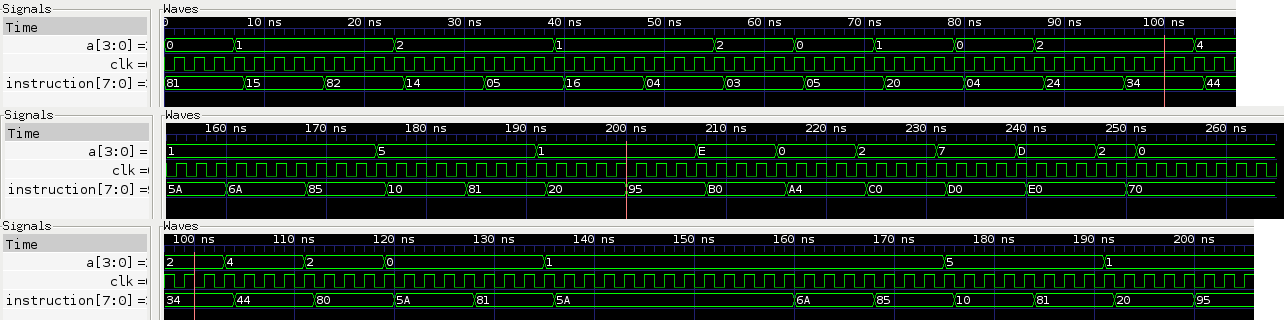
\includegraphics[width=15cm]{figures/sim.png}
  \caption{Simulacion de instrucciones.}
\end{figure}
\begin{figure}[H]
  \centering
  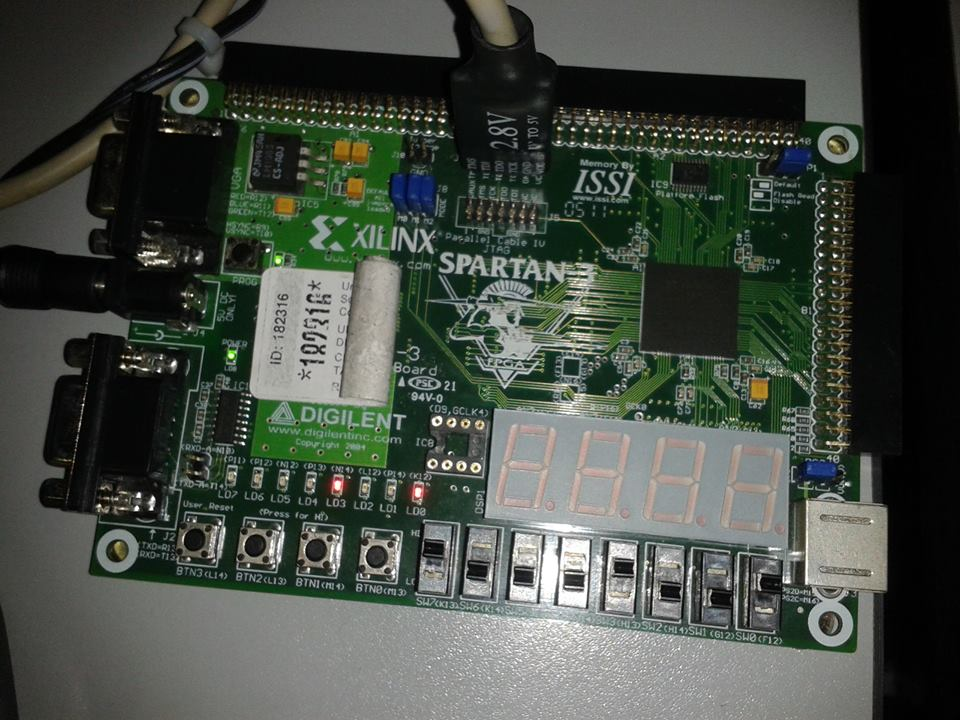
\includegraphics[width=10cm]{figures/2.jpg}
  \caption{Instruccion 0x89.}
\end{figure}
\begin{figure}[H]
  \centering
  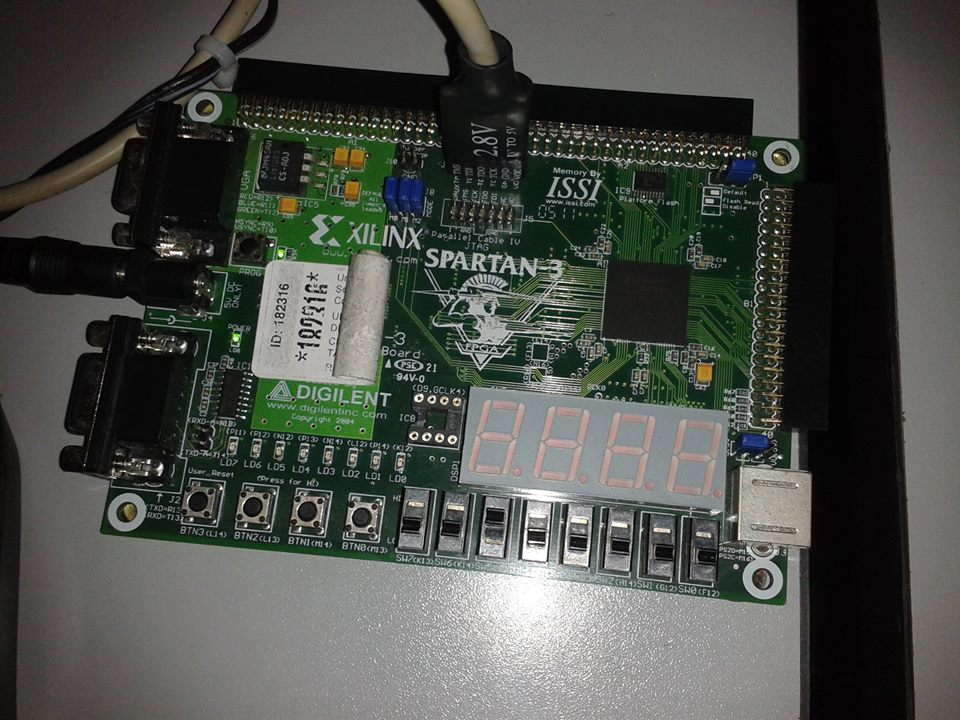
\includegraphics[width=10cm]{figures/4.jpg}
  \caption{Instruccion 0x20.}
\end{figure}
\begin{figure}[H]
  \centering
  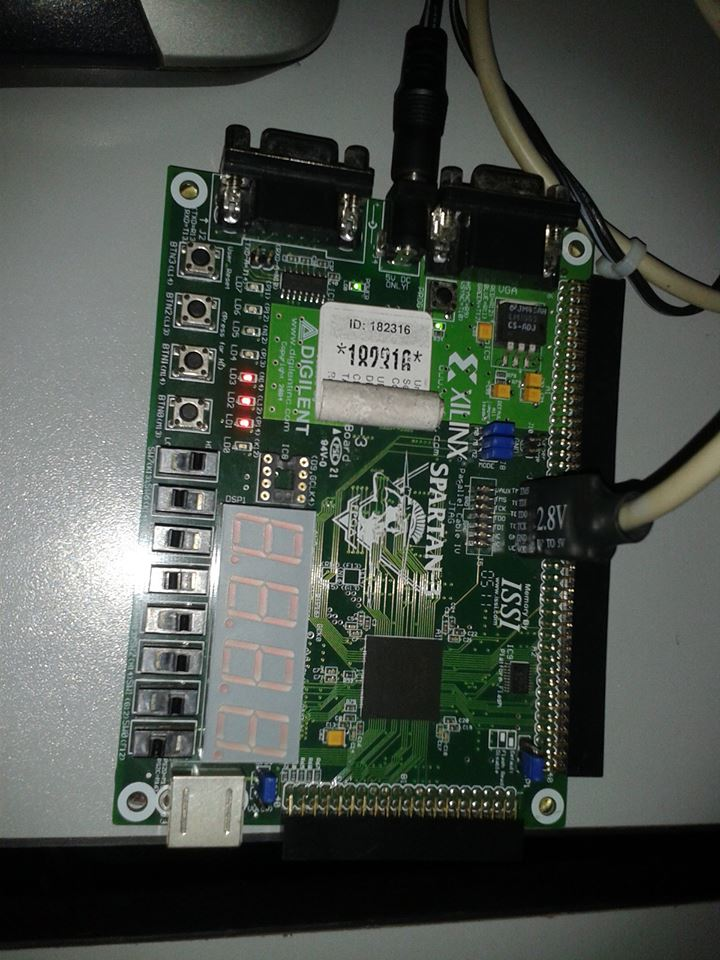
\includegraphics[width=10cm]{figures/3.jpg}
  \caption{Instruccion 0x8E}
\end{figure}


\section{Apéndice}
Documento hecho en \LaTeX . \\
\emph
{
  Para ver los archivos sintetizables ver seccion \textbf{Codigo
    sintetizable} más abajo.
} \\
Los archivos descritos a continuacion son para simularse y utilizarse en
conjunto:= \emph{Linux} (o sistemas basados en Unix) + \emph{Verilator} +
\emph{GTKWave}.\\

\subsection{Makefile}
\textbf{Makefile}
\lstinputlisting{Makefile}

\subsection{cpu.v}
\textbf{cpu.v}
\lstinputlisting{cpu.v}

\subsection{cpu\_tb.cpp}
\textbf{cpu\_tb.cpp}
\lstinputlisting{cpu_tb.cpp}

\subsection{ram.v}
\textbf{ram.v}
\lstinputlisting{ram.v}

\subsection{ram\_tb.cpp}
\textbf{ram\_tb.cpp}
\lstinputlisting{ram_tb.cpp}

\subsection{Codigo sintetizable}
\textbf{ram.v}
\lstinputlisting{ram_s.v}
\textbf{cpu.v}
\lstinputlisting{cpu_s.v}


\end{document}
